\section{Supervised visual learning approach}
\label{mrcnn_section}
This section describes our method for learning to solve geometric problems.
We build on \maskrcnn~\cite{maskrcnn}, a convolutional neural network for the detection and segmentation of objects in images and videos. Given an image, \maskrcnn outputs bounding boxes, segmentation masks, class labels and confidence scores of objects detected in the input image. 

\maskrcnn is a convolutional neural network architecture composed of two modules. The first module is a region proposal network that proposes candidate regions in the image that may contain the target object (e.g. a ``car"). The second module then, given a proposed candidate region, outputs its class (e.g. ``car", ``pedestrian" or ``background"), bounding box, segmentation mask and confidence score.

We adapt the \maskrcnn model for the task of solving geometric construction problems.   
Fig.~\ref{our_approach_schema} shows the diagram of our approach.
The main idea is to train \maskrcnn to predict the tool that should be used at a given step, including its arguments.
For example, as shown in Fig.~\ref{our_approach_schema}, the input is the image depicting the current state of the construction in the red channel of the image (three points in red) and the goal in the green channel (the three sides of the triangle). \maskrcnn predicts here to execute the Line tool. The predicted bounding box of the line is shown in magenta. 
For this purpose, \maskrcnn network has to recognize the two
points in the input image and predict their location, represented by the rectangular masks.
The output masks are then transformed to coordinates of the two points that need to be ``clicked" to execute the Line tool in the Euclidea environment.
 
To train \maskrcnn to solve geometric construction problems, we have to create training data that represent applications of the Euclidea tools and adjust the network outputs to work with our Euclidea environment.
To generate training data for a given Euclidea level, we follow a predefined construction of the level and transform it to match the specific generated level instances (see Section~\ref{sec:euclidea}). Each use of a Euclidea tool corresponds to one example in the training data.
We call each application of a tool in our environment an \emph{action}, represented by the tool name and the corresponding click coordinates.
For example, the Line tool needs two action clicks, representing two points on the constructed line.

The following sections show the generation of training data for \maskrcnn (Section~\ref{sec:action_to_mask}), describe how we derive Euclidea actions from the detected masks at test time (Section~\ref{sec:mask_to_action}), present our algorithm for solving construction problems (Section~\ref{sec:solving_construction}), and introduce additional components that improve the performance of our method (Section~\ref{mrcnn_components}).

\begin{figure}[tbp]
\centering
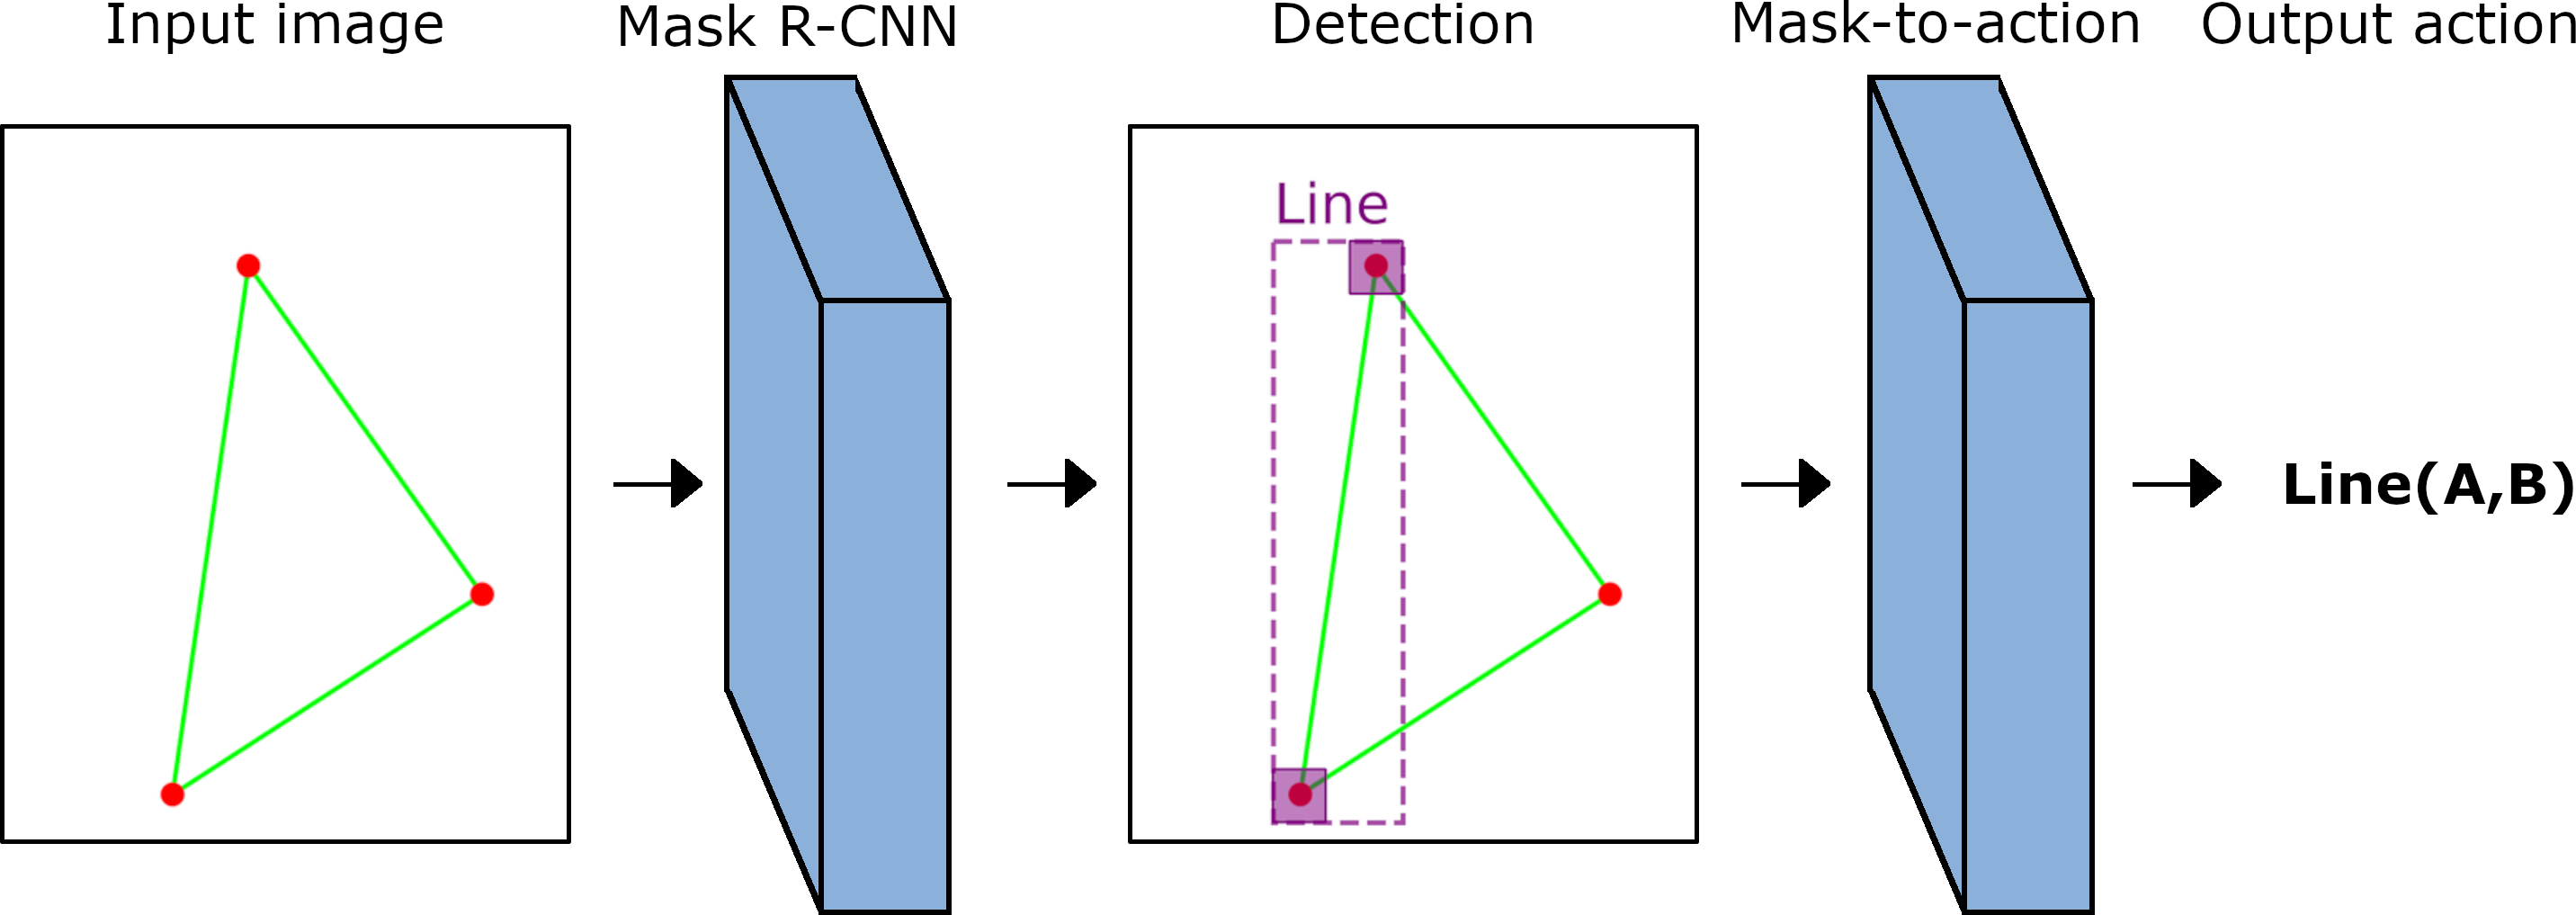
\includegraphics[width=\textwidth]{img/approach_schema_v2.png}
\caption{Diagram of our approach.
The goal is to construct a triangle given three points.
The input is an RGB image with the current state of the construction in the red channel (the three points) and the goal is given in the green channel (the three sides of the triangle).
The \maskrcnn predicts a line between two of the three points.
The dashed rectangle denotes the bounding box of the line and the small square magenta masks denote the two points on the line.
This \maskrcnn line detection is then converted into a Euclidea tool action, $Line(A, B)$, represented by the tool name and its arguments (the locations of the two points).
The process that converts the \maskrcnn output masks into actions in the Euclidea environment is described in Section~\ref{sec:mask_to_action}.}
\label{our_approach_schema}
\vspace*{-1.5em}
\end{figure}

\subsection{Action to Mask: generating training data}
\label{sec:action_to_mask}
Here we explain how we generate the training data for training \maskrcnn to predict the next construction step. In contrast to detecting objects in images where object detections typically do not have any pre-defined ordering, some of the geometric tools have non-interchangeable arguments and we will have to modify the output of \maskrcnn to handle such tools.

We represent the \maskrcnn input as a 256$\times$256 RGB image of the scene with the current state in the red channel and the remaining goal in the green channel; the blue channel contains zeros.
Note that for visualization purposes, we render the black background as white.
Each training example consists of an input image capturing the current state of the construction together with the action specifying the application of a particular tool.
The action is specified by a mask and a class, where the class identifies the tool (or its arguments, see below) and the mask encodes the location of each point click needed for application of the tool in the image, represented as a small square around each click location.
The Perpendicular tool and Parallel tool
have a line as their argument (see Table~\ref{tab:tool_overview}), passed as a mask of either the whole line or one click on the line.

\begin{figure}[ht]
     \centering
     \begin{subfigure}[b]{0.32\textwidth}
         \centering
         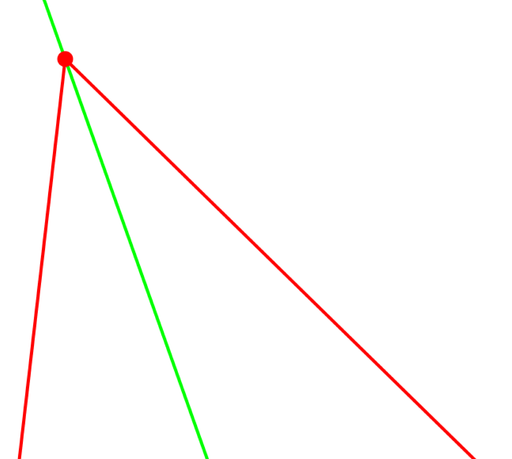
\includegraphics[width=\textwidth]{img/ExampleTrainingData/02_02_input.png}
         \caption{Input}
         \label{fig:training_data_primary_02_02_input}
     \end{subfigure}
     \hfill
     \begin{subfigure}[b]{0.32\textwidth}
         \centering
         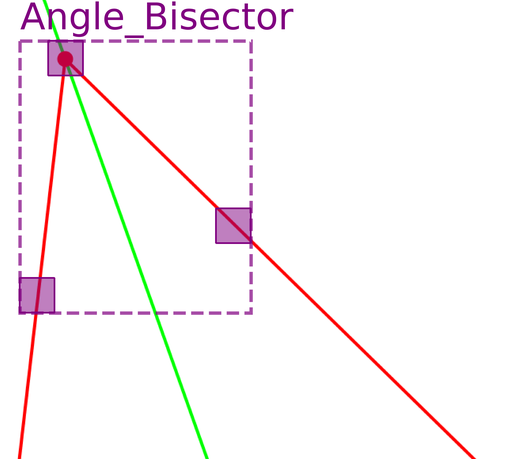
\includegraphics[width=\textwidth]{img/ExampleTrainingData/02_02_primary.png}
         \caption{Primary detection}
         \label{fig:training_data_primary_02_02_primary}
     \end{subfigure}
     \hfill
     \begin{subfigure}[b]{0.32\textwidth}
         \centering
         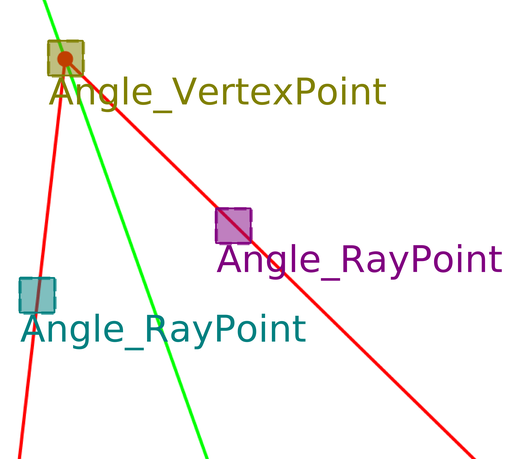
\includegraphics[width=\textwidth]{img/ExampleTrainingData/02_02_secondary.png}
         \caption{Secondary detection}
         \label{fig:training_data_primary_02_02_secondary}
     \end{subfigure}
        \caption{An example from training data for Euclidea level \textit{Beta-02} (construct the line that bisects the given angle).
        The current state is in red and the remaining goal in green.
        (a) Input for the \maskrcnn model.
        (b) Primary detection of the \maskrcnn model identifying the tool type: Angle Bisector tool (purple).
        (c) Three secondary detections identifying the arguments of the tool: one angle vertex point (yellow) and two angle ray points (purple and turquoise).}
        \label{fig:training_data_primary_02_02}
        \vspace*{-1.5em}
\end{figure}

\paragraph{\textbf{Primary and secondary detections.}}
\label{position_dependent_pars}
Encoding clicks as in the previous paragraph is not sufficient for tools with non-interchangeable parameters.
For example, the Circle tool has two non-interchangeable parameters: 1) the center and 2) a point on the circle, defining the radius.
To distinguish such points, we add a secondary output of the \maskrcnn model.
For example, for the Circle tool, we detect not just the circle itself but also the circle center and the radius point.
We denote the detection of the tool (Line tool, Circle tool, ...) as the \emph{primary detection}, and the detection of its parameters as the \emph{secondary detections}.
Fig.~\ref{fig:training_data_primary_02_02} shows an example of primary and secondary detections for the Angle Bisector tool, including the corresponding classes: Angle\_Bisector (primary detection), Angle\_VertexPoint, and Angle\_RayPoint (secondary detections).
\subsection{Mask to Action: converting output masks to Euclidea actions}
\label{sec:mask_to_action}
To solve Euclidea levels, we have to transform the \maskrcnn output to fit the input of the Euclidea environment.
We refer to this step as ``mask-to-action" as it converts the output of \maskrcnn, which is in the form of image masks specifying the primary and secondary detections (see Section~\ref{sec:action_to_mask}), into tool actions in the Euclidea environment.
The mask-to-action conversion consists of two stages. The first stage obtains locations of individual ``point clicks" from the primary detections for the predicted tool and the second stage determines the order of parameters using the secondary detections.

\paragraph{\textbf{First stage:}} To localize individual points, we use the heat map produced by the final \maskrcnn layer.
The heat map assigns each pixel the probability of being a part of the mask and can be transformed into a binary mask by thresholding.
Instead, we use the heat map directly to localize the detected points more accurately.
We select points with the highest probability in the masks using
a greedy non-maximum-suppression method \cite{non_max_sup}.

\paragraph{\textbf{Second stage:}} We will explain this stage on the example of the Angle Bisector tool (see Fig.~\ref{fig:training_data_primary_02_02}).
A detection of this tool has 4 detection outputs from \maskrcnn, namely, 1 primary and 3 secondary detections.
The primary detection corresponds to the whole tool and the secondary detections to the individual points, i.e., one angle vertex point and two angle ray points (see Fig.~\ref{fig:training_data_primary_02_02}).
To use the Angle Bisector tool, we have to determine the correspondence between the primary and secondary detections.
We obtain 3 point coordinates from the primary detection in the first stage, as described above.
We can also get 3 points from the 3 secondary detections, one point per detection.
Each point in the primary detection should correspond to one point in the secondary detection, but these points may not exactly overlap.
The point correspondence is determined by finding a matching between the primary and secondary points that minimizes the sum of distances between the primary and secondary points such that each point is used exactly once.

\subsection{Solving construction problems by sequences of actions}
\label{sec:solving_construction}
Next, we can create an agent capable of solving Euclidea construction problems.
In the previous section, we have described how to get a Euclidea action from \maskrcnn outputs.
However, \maskrcnn can predict multiple candidate detections (that correspond to different actions) for one input image.
\maskrcnn returns for each detection also its score, representing the confidence of the prediction.
To select the next action from the set of candidate actions (derived from \maskrcnn detections) in each step,
the agent follows Algorithm~\ref{alg:top_score_inference}, which chooses the action with the highest confidence score at each state.
\vspace{-6mm}
\begin{algorithm}[!htb]
\SetAlgoLined
\SetAlFnt{\small\sf}
 \KwResult{Test level inference: True if level completed, False otherwise.}
 Initialize a level\;
 \While{level not complete}{
  $s \gets$ current state of the level\;
  $p \gets model.predict(s)$\;
  \If{predictions $p$ are empty}{
   \Return False\;
   }
  $a \gets$ action from $p$ with highest score\;
  execute $a$
 }
 \Return True\;
\vspace{0.5mm}
\caption{\small{Solving construction problems by choosing the action with the highest score.}}
\label{alg:top_score_inference}
\end{algorithm}
\vspace{-8mm}
\subsection{Additional components of the approach}
\label{mrcnn_components}
Here we introduce several additional extensions to the approach described above and later demonstrate their importance in Section \ref{experiments_section}.
\paragraph{\textbf{Automatic point detection.}}
Our Euclidea environment requires that each point important for the solution is identified using the Point tool.
For example, when we have to find the third vertex of the triangle in Fig.~\ref{fig:euclidea_example}, we have to use the Point tool to localize the intersections of the circles.
The Automatic point detection modification automatically adds points to the intersections of objects.
\paragraph{\textbf{History channel.}}
To better recognize which construction steps have already been done and which still need to be constructed, we add a third, history channel (blue) to the input of~\maskrcnn, containing the construction state from the previous step.
\paragraph{\textbf{4+ Stage training.}}
\maskrcnn is typically trained in 2 stages: first, only the head layers are trained, followed by training of the whole network, including the 5-block convolutional backbone.
The 4+ Stage training modification splits the training into 3 stages: first, the head layers are trained, then also the fourth and fifth backbone blocks, and finally, the whole network.
\paragraph{\textbf{Intersection degeneration rules.}}
To decide whether a generated level can be solved using only the image information, we apply the following rules to identify degenerate configurations: a) the radius of a circle cannot be too small, b) the distance between points, lines, or their combinations cannot be too small.
In this modification, we add a third rule: c) any intersection of geometric primitives cannot be too close to points that are necessary for the construction.
This prevents possible alternative solutions from being too close to each other and the auxiliary intersections created during the construction from being too close to points from the initial state and the goal.
\paragraph{\textbf{On-the-fly data generation.}}
Generating training data on-the-fly allows us to (potentially infinitely) expand the training set and thus train better models.

